\chapter{Analyse des besoins}
        Nous débutons la conception de notre système en analysant la
situation pour prendre note des différentes contraintes, des risques
et tout autre élément pertinent dans le but de satisfaire l'intégralité
des besoins de l'URGéo.  Nous sommes déjà imbus du contexte de développement
du système, par conséquent, nous allons, dans cette partie, nous concentrer
sur les besoins et les contraintes de l'application.
\section{Besoins et contraintes}
        Il s'agit de la conception d'une base de données géotechniques et d'une
        application web permettant de visualiser cesdites données. Définissons
        d'abord tous les besoins des différents utilisateurs du système.
        \subsubsection{Identification des acteurs du système}
        Pour connaître les différents besoins des utilisateurs, nous devons
        avant tout relever la liste des différents utilisateurs eux-mêmes.
        Nombreux sont ceux qui auront à utiliser le système. Nous appellerons ces différents
        utilisateurs  les \textbf{acteurs} du système.
        \par
        L'application est disponible pour tout le monde notamment les
        professionnels en géosciences, les ingénieurs, les étudiants, les banques, les 
        compagnies d'assurance, etc.
        Ces acteurs sont divisés en trois (3) catégories:
        \begin{itemize} 
                \item \textbf{les visiteurs: }
                Un visiteur est un utilisateur externe qui se rend sur l'application pour rechercher et visualiser
                les données mises disponibles par l'URGéo et les instances associées. 
              
                \item \textbf{les administrateurs: }
                Un administrateur est un utilisateur interne capable d'interagir directement avec les données. 
                Il a pour principal rôle la gestion des data 
                liés aux différents résultats géotechniques. Tout au long du document, on entendra par data:
                \begin{itemize}
                        \item Les résultats des essais 
                        \item Les fonds de carte
                \end{itemize}
                Il est obligatoire pour lui de s'authentifier pour pouvoir 
                effectuer certaines actions sur le système. Seront administrateurs, toute personne désignée par l'URGéo
                ou les partenaires de l'URGéo. Le plus souvent, il s'agira des stagiares responsables de l'entrée 
                des données.

                \item \textbf{les superadmins: }
                Un super-administrateur est un super utilisateur. Détenant un rôle particulièrement sensible,
                il est obligatoire pour lui de s'authentifier pour y accéder. Ses droits sont particulièrement orientés 
                vers la gestion des ressources du système. Il peut ainsi manipuler les informations relatives aux 
                différents utilisateurs et garder un trace des trafics effectués au sein de l'application.
                 Seront superadmins, toute personne désignée par l'URGéo.
            \end{itemize}   
        \subsubsection{Besoins des différents utilisateurs}
        Étant donné que l'on a deux types d'utilisateurs internes avec des privilèges différents,
        le système doit impérativement comporter un mode de gestion des utilisateurs et des droits d'accès.
        \paragraph{Le visiteur}
        Le visiteur a à sa disposition une carte d'Haïti marquée aux différents endroits où des tests 
        géotechniques ont été réalisés.
        À n'importe quel moment, il peut décider d'effectuer une recherche par mot clé et s'attend
        à ce que le résultat de sa recherche s'affiche sur la carte. Il a aussi l'option de l'afficher sous la forme
        d'une liste qu'il peut filtrer selon son choix. Cette dernière peut être téléchargée sous format CSV.
        En support aux informations spécifiques à un test se trouvant à un endroit bien précis sur la carte,
        le visiteur a aussi l'accès au résultat du test se trouvant dans un fichier PDF qu'il peut télécharger.
        \par
        Aussi, plusieurs fonds de carte seront disponibles permettant au visiteur d'adapter le résultat de ses recherches
        au contexte idéal (topographie, hydraulique,... )
        \par
        Le visiteur peut aussi décider de lire, de commenter ou de laisser un message (de manière anonyme ou pas) 
        sur le forum dédié à l'application.
        \paragraph{L'administrateur}
        Un administrateur ne peut exister sans appartenir à une institution su système. Avant tout, il peut réaliser 
        toutes les actions d'un visiteur. De plus, après s'être authentifié au moyen de 
        son adresse électronique et de son mot de passe, il peut interagir directement avec la base de données. En cas 
        d'oubli de son mot de passe, le système lui envoie un lien de réinitialisation de mot de passe à son email.
        Pour jouer son rôle d'administrateur, il est redirigé vers \textit{l'interface de l'administrateur}. 
        Dans ce module, l'administrateur peut:
        \begin{itemize}
                \item \textbf{Ajouter un test: }
                Il s'agit de rentrer les informations relatives à un test pour l'ajouter dans la base de données.
                Ces informations sont de types différents (nom:texte, identifiant:entier, date du test:date, types
                de test:entier, date d'enregistrement:date, etc\footnote{Les différents champs et leur type seront 
                détaillés dans l'étude des diagrammes à la fin du chapitre} )
                \item \textbf{Modifier un test: }
                Si pour une raison ou pour une autre un test doit être modifié, l'administrateur est en
                mesure de le faire après s'être authentifié. Un message lui sera affiché à l'écran dépendemment 
                de la réussite ou de l'échec de son action. 
                \item \textbf{Supprimer un test: }
                La suppression d'un test est aussi possible. Un message de confirmation précède la validation
                de l'exécution de cette action car elle est irréversible.
        \end{itemize}
        \par
        À noter qu'il ne peut s'aventurer à modifier ou supprimer un test qui n'avait pas été directement 
        ajouté par un administrateur appartenant à la même institution. De plus, si l'URGéo juge que le commentaire d'un visiteur doit être supprimé,
        l'administrateur est apte à réaliser cela.
        \par
        Chaque action effectuée par un administrateur sera enregistrée automatiquement pour permettre la traçabilité
        et la non-répudiation\footnote{On abordera cette partie dans la section sécurité du chapitre 3.}.
        Ainsi, un module permettant de visualiser uniquement les logs\footnote{Historique des actions effectuées sur un 
        système informatique.} du système. Par conséquent, on peut savoir
        la date et l'heure précise où un administrateur ouvre une session, affiche, ajoute, modifie ou supprime une donnée.
        Nul utilisateur ne pourra altérer ces donnéees.
        \par

        \paragraph{Le superadmin}
        Il s'agit là de l'utilisateur de plus haute hiérarchie de notre application. Certes, il est libre 
        d'utiliser l'application comme un simple visiteur. De plus, après s'être authentifié au moyen de 
        son adresse électronique et de son mot de passe, il peut avoir accès tant aux données relatives aux
        différents utilisateurs de son institution qu'au trafic des différentes données en circulation. Il 
        pourra ainsi visionner les statistiques relatives au bien fondé de la plateforme.
        Dans ce module, le superadmin peut:
        \begin{itemize}
                \item \textbf{Ajouter un utilisateur: }
                Il s'agit de rentrer les informations relatives à un utilisateur pour l'ajouter dans la base de données.
                Ces informations sont de types différents (nom:texte, prénom identifiant:entier, type d'utilisateur, 
                etc\footnote{Les différents champs et leur type seront 
                détaillés dans l'étude des diagrammes à la fin du chapitre} )
                \item \textbf{Modifier un utilisateur: }
                Si pour une raison ou pour une autre les informations d'un utilisateur doivent être modifiées, le superadmin est en
                mesure de le faire après s'être authentifié. Un message lui sera affiché à l'écran dépendemment 
                de la réussite ou de l'échec de son action.
                \item \textbf{Activer ou désactiver un utilisateur: }
                Il s'agit d'autoriser ou non un administrateur à utiliser l'application.
                \item \textbf{Visionner la statistique des trafics effectués sur les données de son institution: }
                Un graphe statistique sera mis à sa disposition sans qu'il ne puisse le modifier personnellement.
        \end{itemize}
          

\par    
\begin{table}
        \centering
        \begin{tabular}{|p{0.21\linewidth}|p{0.54\linewidth}|p{0.33\linewidth}|}
        \hline
                \textbf{Utilisateurs} & \textbf{Besoins} & 
                \textbf{Contraintes}  \\
                \hline
                        Visiteur & 
                        \begin{itemize}
                                 \item[$\cdot$]  Cartographie d'Haïti
                                 \item[$\cdot$]  Fonds de carte
                                 \item[$\cdot$]  Recherches
                                 \item[$\cdot$]  Filtrage des donnéees
                                 \item[$\cdot$]  Téléchargement des résultats des tests
                                 \item[$\cdot$]  Navigation simple et attrayante
                        \end{itemize} & 
                        Accès au site à partir du lien \\
                \hline
                        Administrateur & 
                        \begin{itemize}
                                \item[$\cdot$]  Ajout de test
                                \item[$\cdot$]  Modification de test
                                \item[$\cdot$]  Suppression de test
                                \item[$\cdot$]  Suppression de commentaire
                        \end{itemize} & 
                        \begin{itemize}
                                \item[$\cdot$] Authentification 
                                \item[$\cdot$] Appartenance à une institution du système 
                        \end{itemize}
                         \\
                \hline
                        Superadmin & 
                        \begin{itemize}
                                \item[$\cdot$]  Affichage des logs
                                \item[$\cdot$]  Ajout d'administrateur
                                \item[$\cdot$]  Modification d'administrateur
                                \item[$\cdot$]  Activation d'administrateur
                                \item[$\cdot$]  Désactivation d'administrateur
                                \item[$\cdot$]  Accès à l'analyse des flux de l'application 
                        \end{itemize} & 
                        \begin{itemize}
                                \item[$\cdot$] Authentification 
                                \item[$\cdot$] Appartenance à une institution du système 
                        \end{itemize}
                         \\
                \hline  
        \end{tabular}
        \caption{Tableau des utilisateurs et de leurs besoins} \label{tab:sometab}
\end{table}
\par
                \lipsum[1]
        \section{Approche de travail}
        \subsection{Le génie logiciel}
        \textit{
                En 1995, une étude du Standish Group dressait un tableau accablant de la 
                conduite des projets informatiques. Reposant sur un échantillon 
                représentatif de 365 entreprises, totalisant 8 380 applications, 
                cette étude établissait que \cite{audibert2009uml} :
                \begin{itemize}
                        \item 16,2\% seulement des projets étaient conformes 
                        aux prévisions initiales,
                        \item 52,7\% avaient subi des dépassements en coût et délai d'un facteur 2 à 3 
                        avec diminution du nombre des fonctions offertes,
                        \item 31,1\% ont été purement abandonnés durant leur développement.
                \end{itemize}
        }
        \paragraph{}
        GéoTechMap doit faire partie de ces 16,2 \%. Pour ce faire, il ne faut surtout pas
        négliger l'importance du génie logiciel.
        \par
        Le génie logiciel est un domaine de de recherche qui a pour objectif
        d'optimiser le coût de développement d'un logiciel. De ce fait, notre
        travail en tant qu'ingénieurs est de nous occuper de l'architecture
        du logiciel, en l'occurence ses composants ainsi que ses mécanismes.
        La conception passe par plusieurs phases. Ainsi, on établie une approche
        de travail qui permettera de répondre aux besoins grandissants du système 
        que l'on va concevoir.
        \par
        À la suite de l'évaluation et de la documentation des besoins spécifiques
        de l'URGéo, des utilisateurs et des spécifications logiques et matérielles
        relatif au système, un plan a été dréssé:
        \begin{itemize}
                \item l'analyse des besoins,
                \item l'élaboration des spécifications,
                \item la conceptualisation,
                \item le développement,
                \item la phase de test,
                \item déploiement,
                \item vulgarisation,
                \item la maitenance
        \end{itemize}
        \paragraph{Un système de qualité}
        \paragraph{}
        Il s'agira d'offir un logiciel de qualité qui s'appuera sur différents facteurs.
        GéoTechMap rempli exactement les fonction escomptés spécifieés dans le 
        cahier des charges. La validité du système ne pourra être mis en doute.
        De plus, ce sera un une application fiable et robuste, pouvant facilement
        être combiné avec d'autres logiciels (choix de développement API). Dans le 
        Tableau \ref*{tab:facteurs}, figurent les differents facteurs sur lesquels reposent la qualité
        de GéoTechMap.

\par    
\begin{table}
        \centering
        \begin{tabular}{|p{0.20\linewidth}|p{0.80\linewidth}|}
        \hline
                \textbf{Facteurs} & \textbf{Détails} \\
                \hline
                Facilité d'emploi &
                facilité d'apprentissage, d'utilisation, de préparation des données, 
                d'interprétation des erreurs et de rattrapage en cas d'erreur d'utilisation.
                         \\
                \hline
                Validité&
                aptitude d'un produit logiciel à remplir exactement ses fonctions, 
                définies par le cahier des charges et les spécifications
                    \\
                \hline
                Fiabilité &
                aptitude d'un produit logiciel à fonctionner dans des conditions anormales.
                    \\
                \hline
                Réutilisabilité&
                aptitude d'un logiciel à être réutilisé, en tout ou en partie, dans de nouvelles applications.
                    \\
                \hline
                Compatibilité&
                facilité avec laquelle un logiciel peut être combiné avec d'autres logiciels.
                        \\
                \hline
                Efficacité&
                Utilisation optimale des ressources matérielles.
                        \\
                \hline
                Portabilité&
                facilité avec laquelle un logiciel peut être transféré sous différents environnements matériels et logiciels.
                        \\
                \hline
                Vérifiabilité&
                facilité de préparation des procédures de test.
                        \\
                \hline 
                Intégrité&
                aptitude d'un logiciel à protéger son code et ses données contre des accès non autorisés.
                        \\

                \hline 
        \end{tabular}
        \caption{Quelques facteurs sur lesquels reposent la qualité
        de GéoTechMap \cite{audibert2009uml}} \label{tab:facteurs}
\end{table}
\par

        \subsection{Le cycle de vie du logiciel}
        Ce cycle désigne les principales étapes de développement du logiciel.
        Le but de cette sécantation est de permettre la vérification du processus de déveeloppement.
        Il comprend le plus souvent les étapes suivantes :
        \begin{itemize}
                \item L'analyse des besoins et la faisabilité du projet
                \item La conception
                \item Le codage
                \item Les tests
                \item La documentation
                \item La mise en production
                \item La maintenance
        \end{itemize}
        Le cycle de vie peut être modélisé de plusieurs manières (Figure \ref{fig:methv} ).
        Nous utiliserons ici le modèle du cycle en V car demeure actuellement le cycle de vie le 
        plus connu et certainement le plus utilisé. 
        Il s'agit d'un modèle en cascade dans lequel le 
        développement des tests et du logiciel sont effectués 
        de manière synchrone \cite{audibert2009uml}.
        \begin{figure}[ht!]
                \centering
                \begin{subfigure}{.45\linewidth}
                    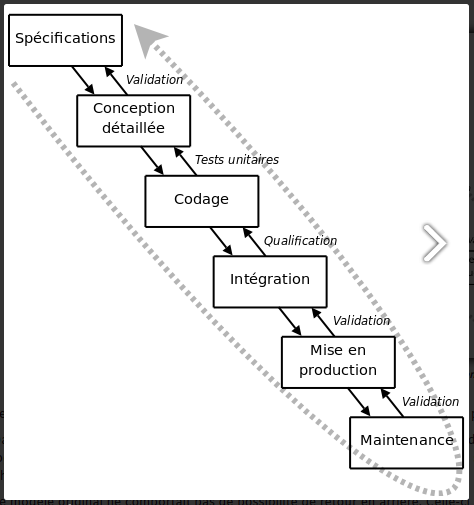
\includegraphics[scale=0.35]{images/Analyse_des_besoins/methcasc.png}
                    \caption{Modèle du cycle de vie en cascade}
                \end{subfigure}
                \hskip2em
                \begin{subfigure}{.45\linewidth}
                    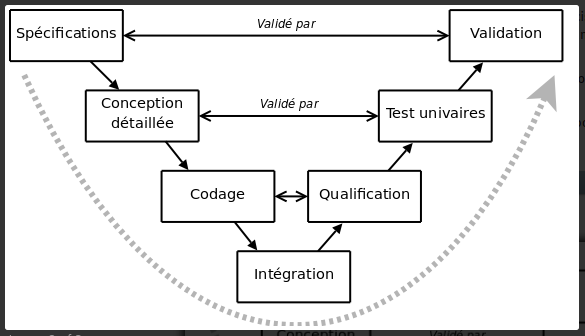
\includegraphics[scale=0.35]{images/Analyse_des_besoins/methv.png}
                    \caption{Modèle du cycle de vie en V}
                    \label{fig:methv}
                \end{subfigure}
               
            \end{figure}
           
       
        \section{Méthodologie}
        Pour la réalisation d'un système complexe, le traitement des problèmes doit se faire 
        de manière efficace. Les tâches lourdes sont divisées en de petites et assignées 
        à chaque membre de l'équipe  en fonction de ses aptitudes à les résoudre. Dans le cadre de ce projet,
        la méthodologie Agile est la plus adaptée.

        \paragraph{Agile, c'est quoi ?}
        \paragraph{}
        \textit{Agile représente un ensemble de “méthodes et pratiques basées sur 
        les valeurs et les principes du Manifeste Agile”, qui repose entre autre sur 
        la collaboration, l’autonomie et des équipes pluri-disciplinaires}\cite{Littlefield2017}.
        \par
        La méthodologie Agile s'oppose généralement à la méthodologie traditionnelle waterfall (en cascade :
        \textit{dès qu'une étape du projet est terminée, l'équipe passe à l'étape suivante ; il n'y a pas (ou peu) 
        de retour en arrière}\cite{david2017}). Elle se veut plus souple 
        et adaptée, et place les besoins du client au centre des priorités du projet.

        \paragraph{Quel framework choisir ?}
        \paragraph{}
        \textit{Ne demandez pas "Kanban vs Scrum". Au lieu de cela, demandez "kanban ou Scrum" 
        ou même "kanban et Scrum"}\cite{Rehkopf}.
        \par
        \paragraph{Scrum}
        \paragraph{}
        \textit{Scrum est un framework qui est utilisé pour implémenter la méthode 
        Agile de développement et de gestion de projet}\cite{Littlefield2017}.
        \par
        Les équipes Scrum s'engagent à livrer les logiciels fonctionnels à des intervalles définis 
        appelés sprints. Leur objectif est de créer des boucles d'apprentissage pour 
        recueillir et intégrer rapidement les commentaires des clients. Les équipes Scrum 
        adoptent des rôles spécifiques, créent des artefacts spéciaux et organisent des cérémonies 
        régulières pour faire avancer les choses. 
        
        \paragraph{Kanban}
        \paragraph{}
        \textit{Kanban est une méthodologie de gestion de projet agile pour le développement de logiciels où l'accent
        consiste à indiquer avec précision le travail à effectuer et le moment où il doit être fait}\cite{skauge}.
        \par
        Kanban consiste à visualiser votre travail, à limiter le travail en cours et à maximiser l'efficacité (ou le flux). 
        Les équipes Kanban se concentrent sur la réduction du temps nécessaire pour prendre un projet (ou une user story) 
        du début à la fin. Ils le font en utilisant un tableau Kanban et en améliorant continuellement leur flux de travail.
        \paragraph{Un mélange de Kanban et de Scrum}
        \paragraph{}
        La méthode agile de gestion de projet et le framework Scrum est basé sur une méthode 
        itérative de livrables du produit. Au lieu d’attendre que le projet soit 100\% finalisé 
        pour le livrer au client, vous délivrez des tronçons “utilisables” du projet au cours du 
        temps. Vous éviterez ainsi de gaspiller des efforts en cas de nécessité de changement ou 
        de problème de communication. Au-delà de l’importance des itérations et des améliorations 
        pour le produit, Scrum s’attache également à améliorer le processus à chaque nouveau cycle.
        \paragraph{}
        Un projet Scrum peut être agencé de différentes manières mais sont toujours présents:
        \begin{itemize}
                \item Product Owner : Il représente les intérêts du client et à ce titre, il a 
                l’autorité pour définir les fonctionnalités du produit final. Dans notre cas, il s'agit de l'URGéo.
                \item Sprint : Scrum utilise des sprints comme intervalles de temps pendant lesquels l’équipe 
                va compléter un certain nombre de tâches. Chaque sprint se termine avec une Rétrospective, qui réunit 
                toute l’équipe afin de partager les retours d’expérience et discuter des améliorations possibles du 
                prochain sprint.
        \end{itemize}

        \paragraph{Pourquoi Agile, Kanban et Scrum ?}
        \paragraph{}
        Nous sommes fixés sur le choix de la méthode Agile. Mais concernant le framework qui va
        l'implémenter, on se fait le plaisir de jongler par moments avec Kanban et Scrum. 
        Le tableau \ref{tab:scrumvskanban} fait une comparaison entre ces deux outils et met l'emphase sur leur convergence.
        \begin{itemize}
                \item Scrum est la méthode agile la plus éprouvée et la plus documentée.
                \item Contrairement à la méthode traditionnelle waterfall, l'approche Agile offre une plus 
        grande flexibilité et une meilleure visibilité dans la gestion du projet. 
                \item Les méthodologies Kanban sont continues et plus fluides, tandis que Scrum est basé 
                sur des sprints de travail courts et structurés (qui nous est necessaire par moment).
                \item L'avantage majeur de l'approche Agile est sa flexibilité. Les changements du client et les imprévus 
        sont pris en compte et l'équipe projet peut réagir rapidement.
                \item Le client dispose d'une meilleure visibilité sur l'avancement du projet et peut ainsi l'ajuster 
                en fonction de ses besoins. Le contrôle qualité est permanent. Quant à l'équipe projet, elle peut 
                réagir rapidement aux demandes du client.
                \footnote{
                \url{https://www.planzone.fr/blog/quest-ce-que-la-methodologie-agile}
                }
        \end{itemize}

        \par    
\begin{table}
        \centering
        \begin{tabular}{|p{0.20\linewidth}|p{0.40\linewidth}|p{0.40\linewidth}|}
        \hline
                \textbf{} & \textbf{Scrum}& \textbf{Kanban}  \\
                \hline
                Cadence &
                Sprints réguliers de longueur fixe (ex: 2 semaines)&
                Flux continu
                \\
                \hline
                Méthodologie de publication&
                À la fin de chaque sprint&
                Livraison continue
                    \\
                \hline
                Roles &
                Product owner, scrum master, development team&
                Aucun rôle requis
                    \\
                \hline
                Indicateurs clés&
                Rapidité&
                Délai d'exécution, temps de cycle, WIP(Work In Progress)
                    \\
                \hline
                Philosophie de changement&
                Les équipes ne doivent pas apporter de modifications pendant le sprint.&
                Le changement peut survenir à tout moment
                        \\

                \hline 
        \end{tabular}
        \caption{Comparaison de Scrum et Kanban} \label{tab:scrumvskanban}
\end{table}
\par
        
        
        

        \section{Structure modulaire}
                Le dictionnaire Larousse définit une stucture modulaire comme suit : 
                \textit{Se dit d'un système, matériel ou logiciel, conçu en séparant les 
                fonctions élémentaires pour qu'elles puissent être étudiées et réalisées séparément}\cite{Larousse}. 
                Cette décision est prise pour faciliter la conception et l'évolution du système GéotechMap.
                On réalisant des modules indépendant, il devient plus facile de les tester, les modifier 
                ainsi que les intégrer dans d'autres applications. Par conséquent, la communication entre les modules 
                est plus fluide et n'importe quel ingénieur que travailler sur le sytème.
                \paragraph{Les pricipaux modules sont :}
                \begin{itemize}
                        \item La base de données
                        \item Les API
                        \item La gestion des utilisateurs
                        \item L'administration
                        \item Le côté client
                \end{itemize}
                \paragraph{La base de données}
                \paragraph{}
                Une base de données est un ensemble d'informations organisées de manière 
                à être facilement accessibles, gérées et mises à jour. Il existe les types de bases de données:
                \begin{itemize}
                        \item Base de données centralisée.
                        \item Base de données distribuée.
                        \item Base de données personnelle.
                        \item Base de données relationnelle.
                        \item ...\footnote{https://www.tutorialspoint.com/Types-of-databases}
                \end{itemize}
                Notre choix est axé sur la base de données relationnelle (plus de détails dans le chapitre suivant).
                Ces bases de données sont catégorisées par un ensemble de tables où les données 
                sont intégrées dans une catégorie prédéfinie. La table se compose de lignes (tuples)
                et de colonnes où la colonne a une entrée pour les données d'une catégorie spécifique 
                et les lignes contiennent une instance pour ces données définies en fonction de la catégorie. 
                Le langage SQL (Structured Query Language) est le langage standard pour interagir avec
                 une base de données relationnelle.
                 \paragraph{}
                 \textit{Le modèle relationnel simple mais puissant est utilisé par des organisations 
                 de tous types et de toutes tailles pour une grande variété de besoins d'information}\cite{Oracle}.
                  Les bases de données relationnelles sont utilisées pour suivre les inventaires, 
                  traiter les transactions de commerce électronique, gérer d'énormes quantités d'informations
                   client critiques, et bien plus encore. Une base de données relationnelle peut être envisagée 
                   pour tout besoin d'information dans lequel les points de données sont liés les uns 
                   aux autres et doivent être gérés de manière sécurisée, basée sur des règles et cohérente.

                \paragraph{Les API}
                \paragraph{}
                \textit{Une API est un ensemble de définitions et de protocoles qui facilite la création et 
                l'intégration de logiciels d'applications}\cite{RedHat}. API est un acronyme anglais qui signifie 
                « Application Programming Interface », que l'on traduit par interface de programmation d'application.
                \paragraph{Utilité :}
                Les API permettent à votre produit ou service de communiquer avec d'autres produits et services 
                sans connaître les détails de leur mise en œuvre. Elles simplifient le développement d'applications 
                et vous font ainsi gagner du temps et de l'argent. Lorsque vous concevez de nouveaux outils et produits, 
                ou que vous assurez la gestion de ceux qui existent déjà, les API vous offrent plus de flexibilité, 
                simplifient la conception, l'administration et l'utilisation, et vous donnent les moyens d'innover.
                \textit{Les API sont parfois considérées comme des contrats, avec une documentation qui constitue 
                un accord entre les parties : si la partie 1 envoie une requête à distance selon une structure 
                particulière, le logiciel de la partie 2 devra répondre selon les conditions définies. 
                Chaque partie s’engage à respecter le contrat, donnant ainsi de la stabilité aux échanges}\cite{Alteva}
                \paragraph{}
                Les API Web utilisent en général le protocole HTTP pour leurs messages de requête et fournissent une 
                définition de la structure des messages de réponse. Les messages de réponse se présentent 
                la plupart du temps sous la forme d'un fichier XML ou JSON. Ces deux formats sont les plus courants, 
                car les données qu'ils contiennent sont faciles à manipuler pour les autres applications.
                \paragraph{La gestion des utilisateurs}
                \paragraph{}
                On fait en sorte que la gestion des utiliateurs soit indépendant de l'application.
                Cela allège l'application. De plus, à n'importe quel moment, de nouvelles règles peuvent être définies
                pour les utilisateurs. Ce module est hébergé sur une instance à part et délivre ses services.
                \paragraph{L'administration (Dashboard admin)}
                \paragraph{}
                La partie administration est une application à part entière qui communique avec la base de données.
                Différents modules sont implémentés: Essais, Institutions, etc. Cette partie est constitué du controlleur
                en backend et d'un interface utiliateur.
                \paragraph{Le côté client}
                

        \section{Préparation des documents}
                

                \par
                Étant donnée que la majorité des rapports et résultats des tests sont 
                disponibles sous forme papier, la première étape a consisté à scanner les documents.
                Pour ce faire nous adoptons une protrocole: on assure la traçabilité de chaque 
                document les munissant d'une cartouche reprennant une série d'informations.
                Voici la liste des informations qui forme une cartouche:
                \begin{itemize}
                        \item \textbf{Lieu: }
                        Il s'agit de l'endroit où l'étude a été effectuée.
                        \item \textbf{Date: }
                        Il s'agit de la date à laquelle l'étude a été effectuée.
                        \item \textbf{Maître d'ouvrage: }
                        Il s'agit du client pour lequel l'étude est effectuée.
                        \item \textbf{Maître d'œuvre : }
                        Il s'agit de la personne ou l'entreprise chargée de l'étude.
                        \item \textbf{Réf Numéro Étude: }
                        Il s'agit d'un identifiant unique permettant de tracer une étude.
                \end{itemize}
                
\par    
\begin{table}
        \centering
        \begin{tabular}{|p{0.30\linewidth}|p{0.40\linewidth}|}
                \hline
                \textbf{Lieu} & Delmas \\
                \hline
                \textbf{Date} & Janvier 2020 \\
                \hline
                \textbf{Maître d'ouvrage} & Faculté Des Sciences \\
                \hline
                \textbf{Maître d'œuvre} & URGéo \\
                \hline
                \textbf{Réf Numéro Étude} & 1234 \\
                \hline
        \end{tabular}
        \caption{Exemple de cartouche sur un document d'étude géotechnique} \label{tab:example_cartouche}
\end{table}
\par

        \section{Modélisation avec UML}
        
\paragraph{Pourquoi modéliser ?}
\paragraph{}
La modélisation est le fait de représenter de manière abstraite et simplifiée
une entité du monde réel. Cette entité peut être un phénomène, un processus ou 
comme dans notre cas, un système. L'objectifif de la modélisation est de décrire
, d'analyser, d'expliquer ou de prévoir l'evolution de l'entité en question.
\paragraph{}
Le modèle est enfin indispensable pour assurer un bon niveau de qualité 
et une maintenance efficace. Le choix du modèle a donc une influence capitale 
sur les solutions obtenues.
\paragraph{UML}
\paragraph{}
Une image vaux mieux que milles mots.
Considérez que ce proverbe comme le résumé de l'origine
de la schématisation en langage de modlisation unifié.
Le langage UML (Unified Modeling Language) résume et visualise les 
systèmes de programmation orientés objet. UML est un langage de 
modélisation orienté objet, c’est-à-dire que toutes 
les entités modélisées sont des objets ou se rapportent à des 
objets \cite{conan}.

Son objectif est de créer un langage visuel commun dans le monde 
complexe du développement de logiciels. Il serait aussi comprehensible
par les professionnels et ceux qui veulent comprendre un système. 
\paragraph{}
Le Unified Modeling Language spécifie 14 types de 
diagrammes qui représentent la structure, le comportement et les interactions d’un système.
\subsection{Diagrammes des cas d'utilisation}
    \subsubsection{Cas général}
    \paragraph{}
    \begin{figure}
        \centering
        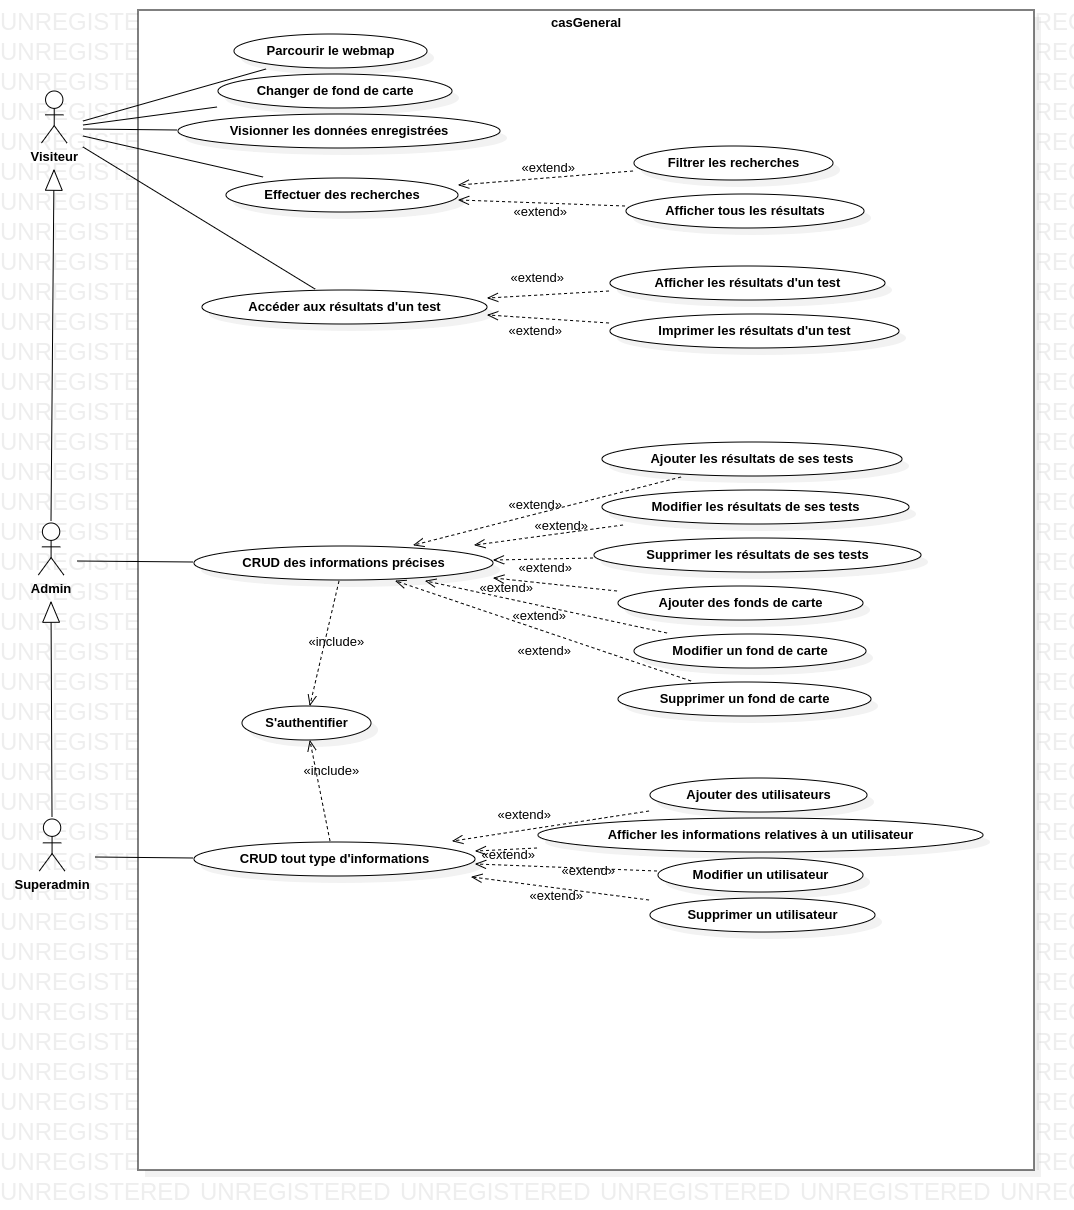
\includegraphics[width=1\textwidth]{images/Analyse_des_besoins/casGeneral.png}
        \caption{Diagramme des cas d'utilisation général}
    \end{figure}
    \par 
    Trois niveaux d'acteurs sont à considérer au sein du système: un visiteur, 
    un administrateur et un super administrateur. La hiérarchisation permet que 
    chaque niveau ait accès aux droits du niveau immédiatement inférieur. 
    De ce fait, un super administrateur est également un administrateur et 
    un visiteur en plus de son niveau direct. \par 
Pour commencer, le visiteur a des droits d'accès très restreints: \par 
\begin{itemize}
    \item Parcourir le webmap: Le visiteur peut voir l'ensemble des informations 
    géotechniques disponibles sur la carte.
    \item Changer de fond de carte: Afin de mieux illustrer le contexte marquant 
    l'intérêt du visiteur, une variété de fonds de carte est accessible sur le site. 
    Ainsi, l'utilisateur peut puiser dans le champs de choix qui lui sont proposés.
    \item Visionner les données enregistrées: En cliquant sur une légende précise, 
    le visiteur peut voir les données qui ont été préalablement enregistrées dans la base de données.
    \item Effectuer des recherches: Deux options s'offrent aux utilisateurs. Ces derniers 
    peuvent afficher tous les résultats au cours de la rechercherche, ou encore ils peuvent 
    se fixer des filtres capables de mieux limiter les plages des résultats.
    \item Accéder aux résultats d'un test: Une fois les résultats obtenus, le visiteur 
    peut soit simplement les afficher, soit les imprimer.
\end{itemize}

\paragraph{}
De son côté, l'\textbf{administrateur} s'occupe de la gestion des informations au sein de la base 
de données. En plus des droits de visiteur, ce type d'utilisateur peut:
\begin{itemize}
    \item Ajouter des informations géotechniques: L'admin peut ajouter des informations 
    dans la bdd, qui sont reflétées sur la carte. 
    \item Modifier les informations qu'il avait préalablement enregistrées: Il ne peut 
    modifier que les informations qu'il avait lui-même ajoutées.
    \item Supprimer les informations qu'il avait préalablement enregistrées: Tout comme il 
    en est pour la modification, il ne peut supprimer que les informations qu'il avait lui-même ajoutées.
    \item Ajouter un fond de carte
    \item Supprimer un fond de carte
\end{itemize}

\par 
Évidemment, aucune de ces actions ne saura avoir lieu tant que l'administrateur ne s'est pas authentifié.

En dernier lieu, le super administrateur joue surtout un rôle de gestionnaire en ressources 
humaines. Une fois authentifié, en plus des droits d'accès d'un simple administrateur, 
cet utiliateur peut:
\begin{itemize}
    \item Ajouter des utilisateurs
    \item Modifier les utilisateurs
    \item Afficher les informations relatives aux différents utilisateurs, pouvant 
    ainsi retracer toutes les actions posées par un utilisateur du système.
    \item Supprimer ou désactiver un utilisateur: La différence se fait remarquer 
    par le fait que le super admin peut supprimer complètement un utilisateur ainsi 
    que toutes les informations y relatives ou simplement désactiver le compte d'un 
    utilisateur sans, pour autant, éliminer ses données.
\end{itemize}

\subsubsection{Parcourir le Webmap}
    \paragraph{}
    \begin{figure}
        \centering
        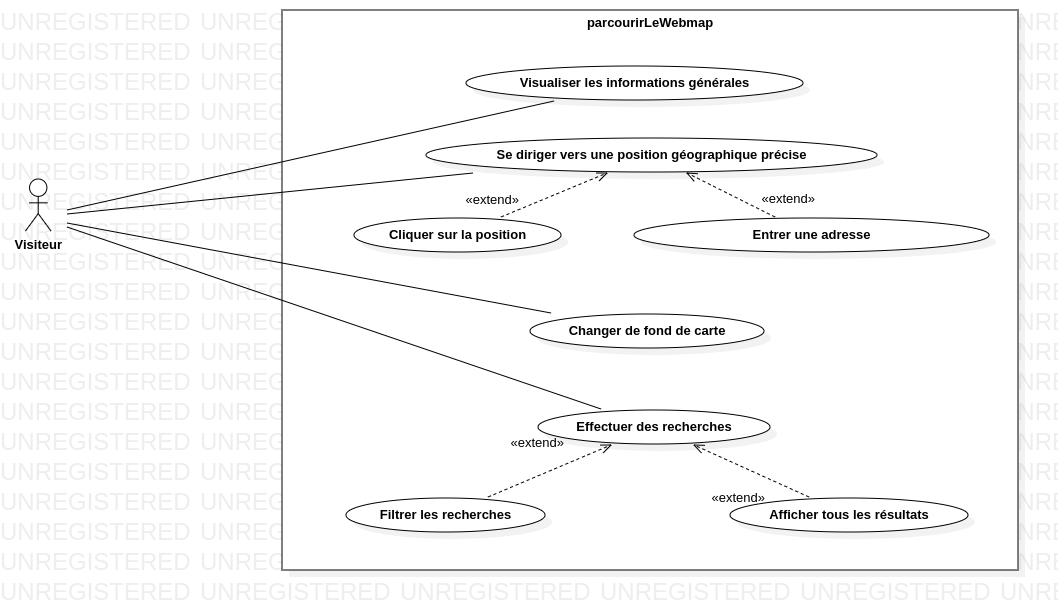
\includegraphics[width=1\textwidth]{images/Analyse_des_besoins/parcourirLeWeb.png}
        \caption{Diagramme du parcours du webmap}
    \end{figure}
\par 
Tout individu, concernés ou pas, par les informations fournies par 
le webmap peut parcourir l'application. Pour ce faire, aucune authentification 
n'est nécessaire au préalable. Lorsqu'un visiteur accède au site, il peut donc:
\begin{itemize}
    \item \textbf{Visualiser les informations générales:}
    Les informations sont disponibles sur une carte pouvant être interprétés
    par un particulier. Elles sont étiquetées sur les points géographiques respectives.
    De ce fait, il peut sélectionner une étiquette particulière afin d'avoir 
    accès à ces données, lui permettant de 
    \begin{itemize}
        \item Visualiser le fichier pdf
        \item Télécharger ce fichier
    \end{itemize}
    \par 
    À première vue, le visiteur ne voit que la carte remplie de 
    "pin[MPOKO JWENN TERME FRANCAIS A]" colorés relatifs à une légende 
    explicite pour la compréhension du visiteur. En plus des légendes, une liste 
    de wigdets facilitant la navigation de l'utilisateur.
    \item \textbf{Accéder à une position géographique précise}
    Toutes les informations étant disponibles, le visiteur peut choisir 
    de visualiser les données relatives à une position bien définies. Pour y accéder, il 
    peut:
    \begin{itemize}
        \item Cliquer directement sur la position géographique
        \item Entrer une adresse dans le champs y frelatif
    \end{itemize}
    \item \textbf{Changer de fond de carte}
    Chaque individu visite ce webmap dans un contexte personnel. Par 
    ailleurs, il peut changer le fond de la carte en fonction de 
    ses besoins. Ces images peuvent varier d'un point de vue hydraulique
    à un point de vue magmatique en passant par tous les fonds mis 
    à la disposition de l'utilisateur par les institutions.
    \item \textbf{Effectuer des recherches relatives aux essais}
    Grand nombre d'essais sont enregistrés sur la carte. Pour faciliter 
    la navigation, une possibilité de recherche est offerte. Dans ce cas,
    il peut donc:
    \begin{itemize}
        \item Afficher tous les résultats
        \item Filtrer les recherches 
    \end{itemize}
\end{itemize}

\subsubsection{Manipulation des données de la base}
    \paragraph{}
    \begin{figure}
        \centering
        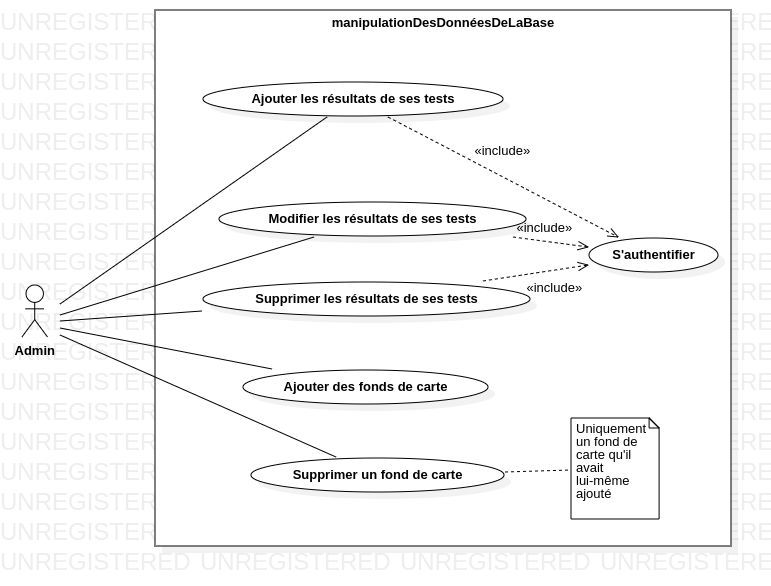
\includegraphics[width=1\textwidth]{images/Analyse_des_besoins/manipulationDesDonneesDeLaBase.png}
        \caption{Diagramme de la manipulation des données de la base}
    \end{figure}
    \par 
    Avant même que les données puissent être disponibles et interprétables 
    par un utilisateur, il faut qu'elles soient intégrées et manipulées continuellement. Le 
    seul utilisateur ayant habilité à faire de telles 
    actions est l'administrateur. Néanmoins, il ne peut manipuler que les informations 
    qu'il a lui-même insérées dans la base de données. Ces dernières étant sensibles, L'admin 
    doit s'authentifier avant d'avoir des droits d'accès à toute sorte de manipulation.

    \subsection{Diagramme de classes}
    \paragraph{}
    Il s'agit du diagramme le plus important dans le cadre 
    d'une modélisation orientée objet. Grâce à lui, le concepteur peut 
    représenter la structure interne du travail à réaliser, lui 
    permettant de trouver un meilleur terrain d'entente avec le client.
    \par 
    Trois grandes classes sont donc implémentées:
    \begin{itemize}
        \item Utilisateur
        \item Institution
        \item Essai 
    \end{itemize}
    \par 
    [TO BE CONTINUED - Take a look ds le fichier mdj]

    \subsection{Diagramme d'objets}
    \paragraph{}
    Ce diagramme \ref{fig:ObjectDiagram} montre les relations entre des objets à travers 
    des exemples tirés du monde réel et permet de voir 
    l'apparence d'un système à n'importe quel instant donné. 
    Les données sont disponibles à l'intérieur des objets, 
    elles peuvent donc être utilisées pour clarifier les 
    relations entre des objets.
    \paragraph{}
    Un diagramme d'objets représente des objets (i.e. instances 
    de classes) et leurs liens (i.e. instances de relations) 
    pour donner une vue figée de l'état d'un système à un 
    instant donné. Un diagramme d'objets peut être utilisé pour :
    \begin{itemize}
        \item illustrer le modèle de classes en montrant un exemple qui explique le modèle ;
        \item  préciser certains aspects du système en mettant en évidence des détails imperceptibles dans le diagramme de classes ;
        \item exprimer une exception en modélisant des cas particuliers ou des connaissances non généralisables qui ne sont pas modélisés dans un diagramme de classe ;
        \item prendre une image (snapshot) d'un système à un moment donné.
    \end{itemize}
    Le diagramme de classes modélise les règles et le diagramme d'objets 
    modélise des faits \cite{audibert2009uml}.
    \begin{figure}[t]
        \centering
        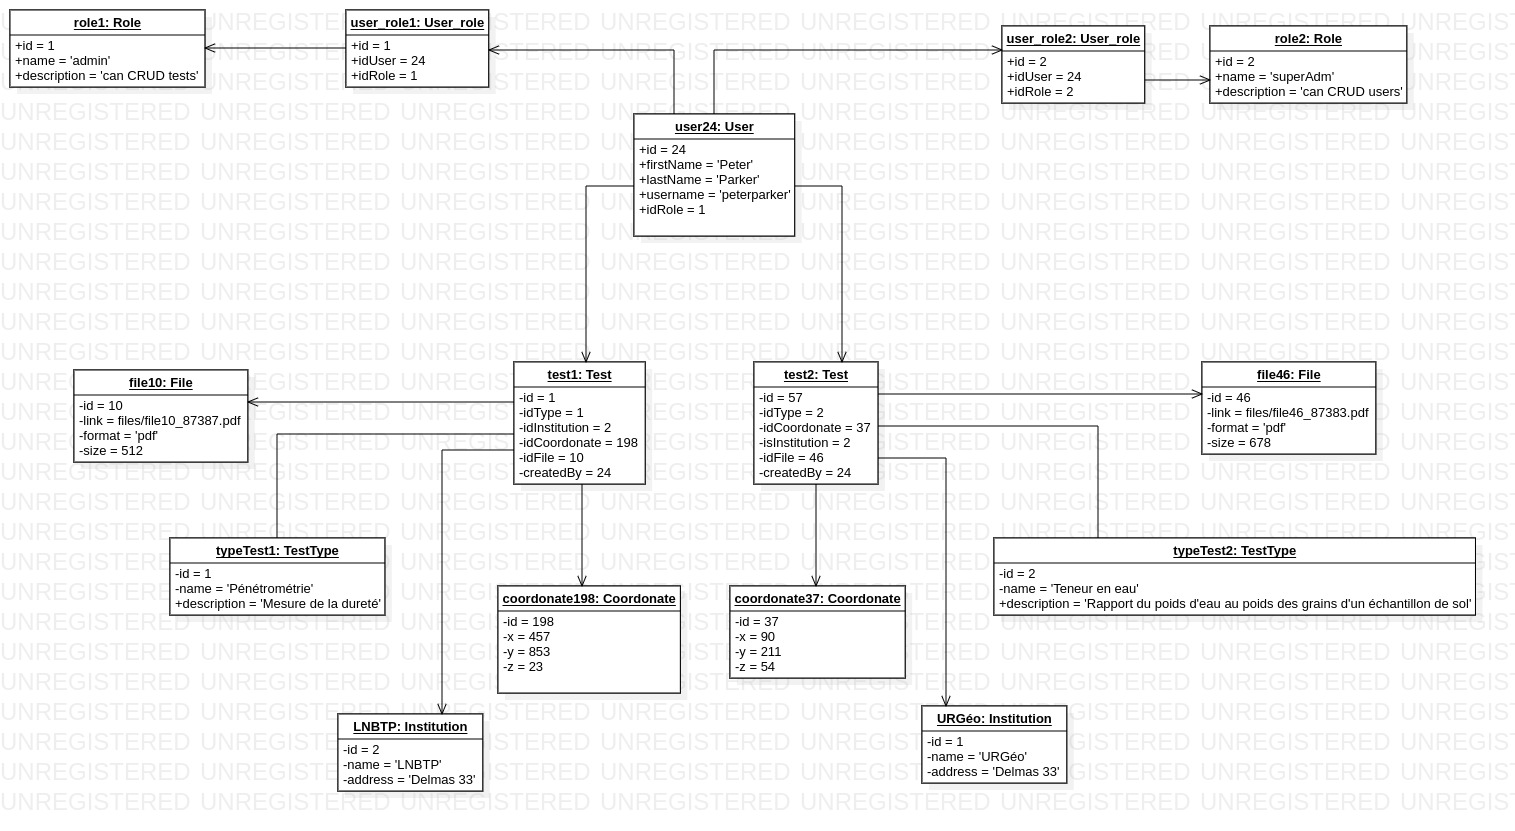
\includegraphics[width=1\textwidth]{images/Analyse_des_besoins/ObjectDiagram.jpg}
        \caption{Cheminement de la solution}
        \label{fig:ObjectDiagram}
    \end{figure}

    \subsection{Diagramme d'activités}
    Le diagramme d'activités a pour rôle principal de représenter graphiquement 
    le comportement du système. Il facilite ainsi la compréhension de chacun en prenant 
    en compte l'interaction des acteurs tant internes qu'externes. 
    \par 
    Dans le cadre d'un projet d'automatisme, nous nous serions probablement tournés vers un 
    diagramme d'états-transitions qui saurait prendre en compte chaque état du système afin d'en prévenir
    la prochaine action. Mais là, l'interaction obligatoire d'un acteur nous oblige à 
    considérer le comportement d'un système basé sur la programmation orientée objet. Il 
    montre les actions à un très haut niveau d’abstraction avec les interactions entre elles \cite{conan2015introduction}. 
    Notre diagramme se présente alors comme suit:
    

    \subsection{Diagramme de séquence}
    Les diagrammes de séquence sont une solution de modélisation 
    dynamique populaire dans UML car ils se concentrent spécifiquement 
    sur les lignes de vie, ou les processus et les objets qui vivent 
    simultanément, et les messages échangés entre eux pour exécuter 
    une fonction avant la fin de la ligne de vie. 
    \par
    Un diagramme de séquence est un type de diagramme d'interaction car 
    il décrit comment et dans quel ordre un groupe d'objets fonctionne 
    ensemble. Ces diagrammes sont utilisés par les développeurs de 
    logiciels et les professionnels pour comprendre les exigences 
    d'un nouveau système ou pour documenter un processus existant. 
    Les diagrammes de séquence sont parfois appelés diagrammes d'événements 
    ou scénarios d'événements.
    \par 
    Le but principal d'un diagramme de séquence est de définir des séquences 
    d'événements qui aboutissent à un résultat souhaité. L'accent est moins mis 
    sur les messages eux-mêmes que sur l'ordre dans lequel les messages se produisent; 
    néanmoins, la plupart des diagrammes de séquence communiqueront quels messages sont 
    envoyés entre les objets d’un système ainsi que l’ordre dans lequel ils se 
    produisent \cite{citeseqdiag}.
    \paragraph{}
    \textit{Les principales informations contenues dans un sont les messages échangés 
    entre les lignes de vie, présentés dans un ordre chronologique. Ainsi, 
    contrairement au diagramme de communication, le temps y est représenté 
    explicitement par une dimension (la dimension verticale) et s'écoule de 
    haut en bas\cite{}.}
    \begin{figure}[t]
        \centering
        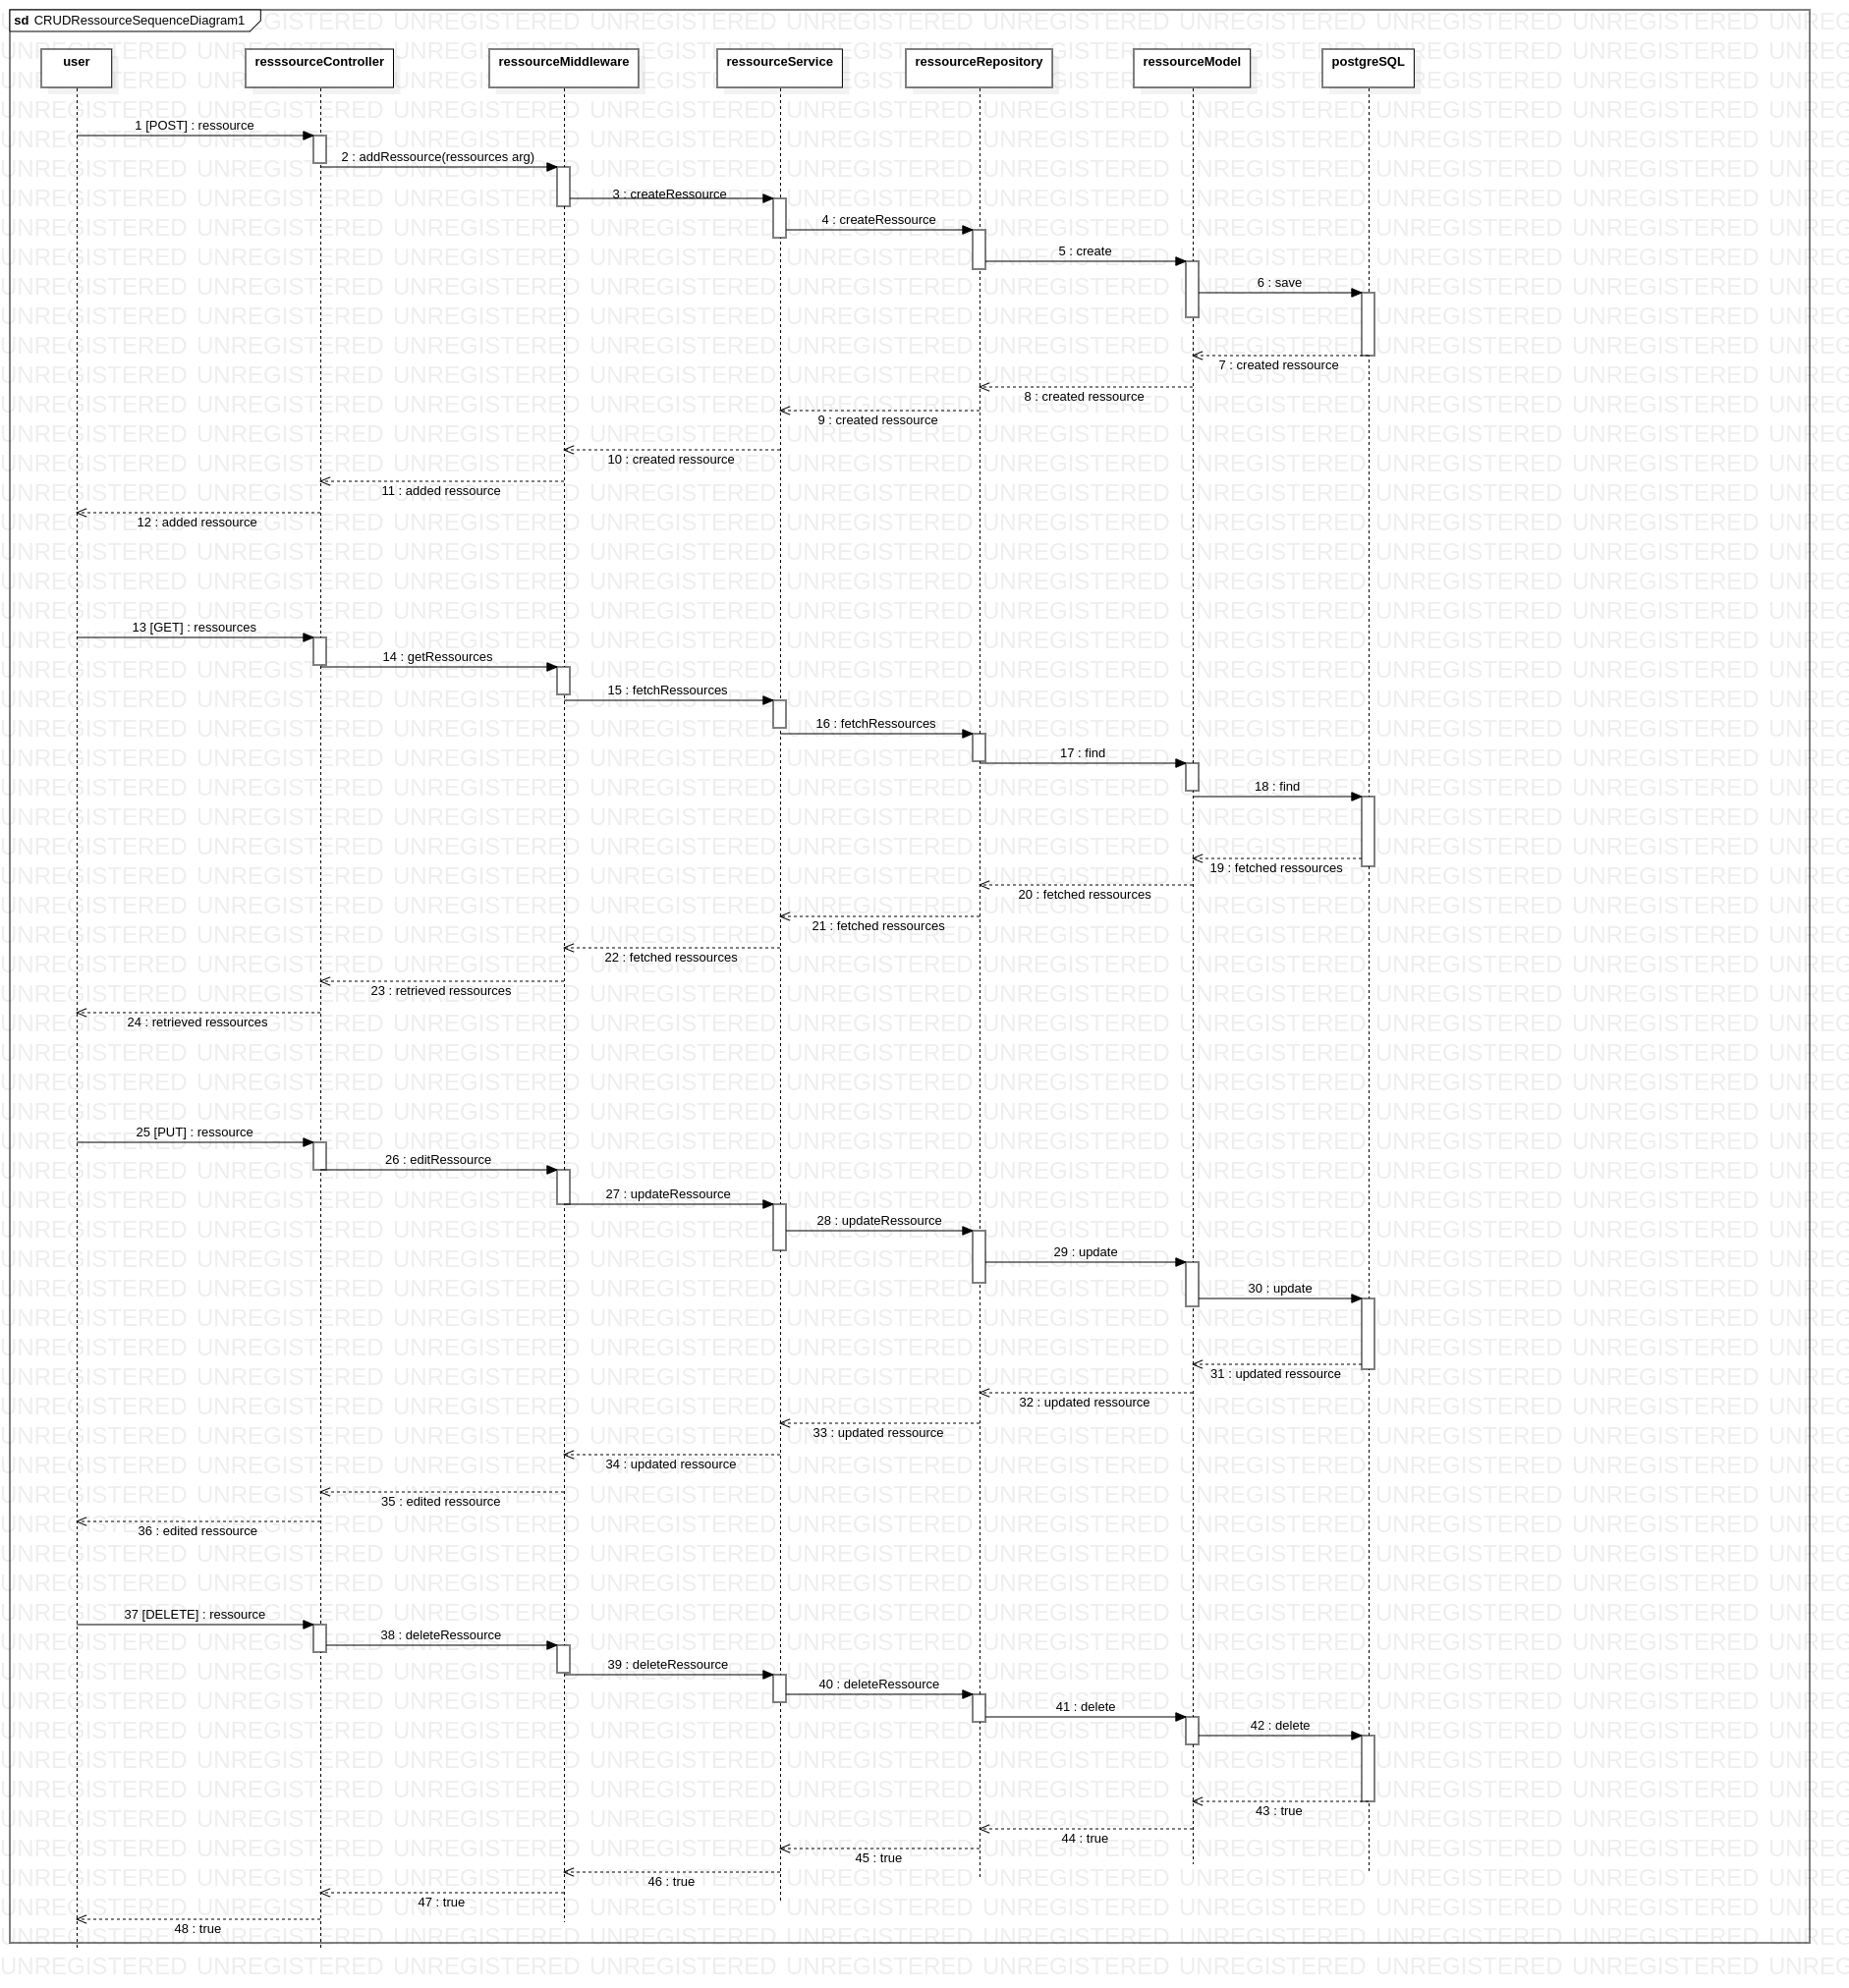
\includegraphics[width=1\textwidth]{images/Analyse_des_besoins/CRUDRessourceSequenceDiagram1.png}
        \caption{Diagramme des séquences : CRUD ressources}
        \label{fig:CRUDRessourceSequenceDiagram1}
    \end{figure}

    \begin{figure}[t]
        \centering
        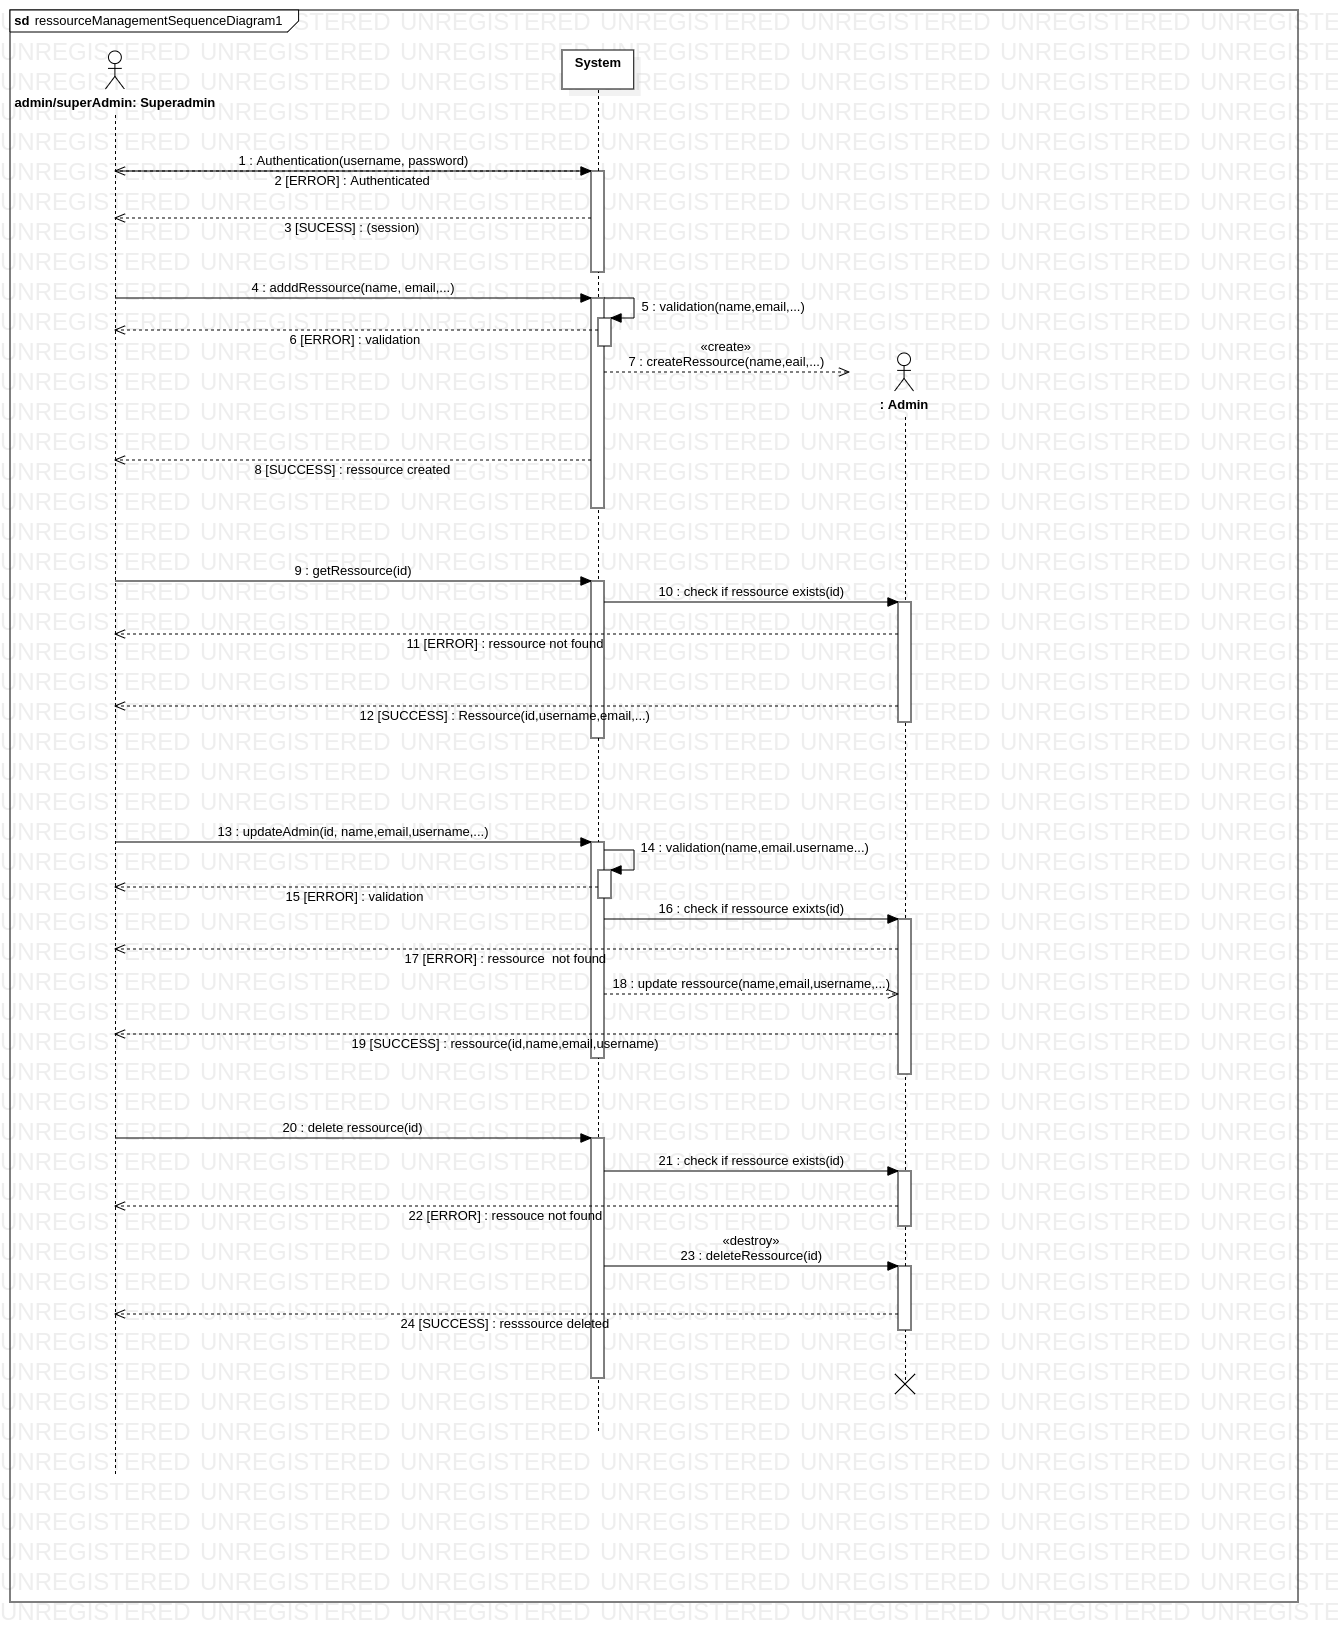
\includegraphics[width=1\textwidth]{images/Analyse_des_besoins/ressourceManagementSequenceDiagram1.png}
        \caption{Diagramme des séquences : gestion des ressources}
        \label{fig:ressourceManagementSequenceDiagram1}
    \end{figure}

    \begin{figure}[t]
        \centering
        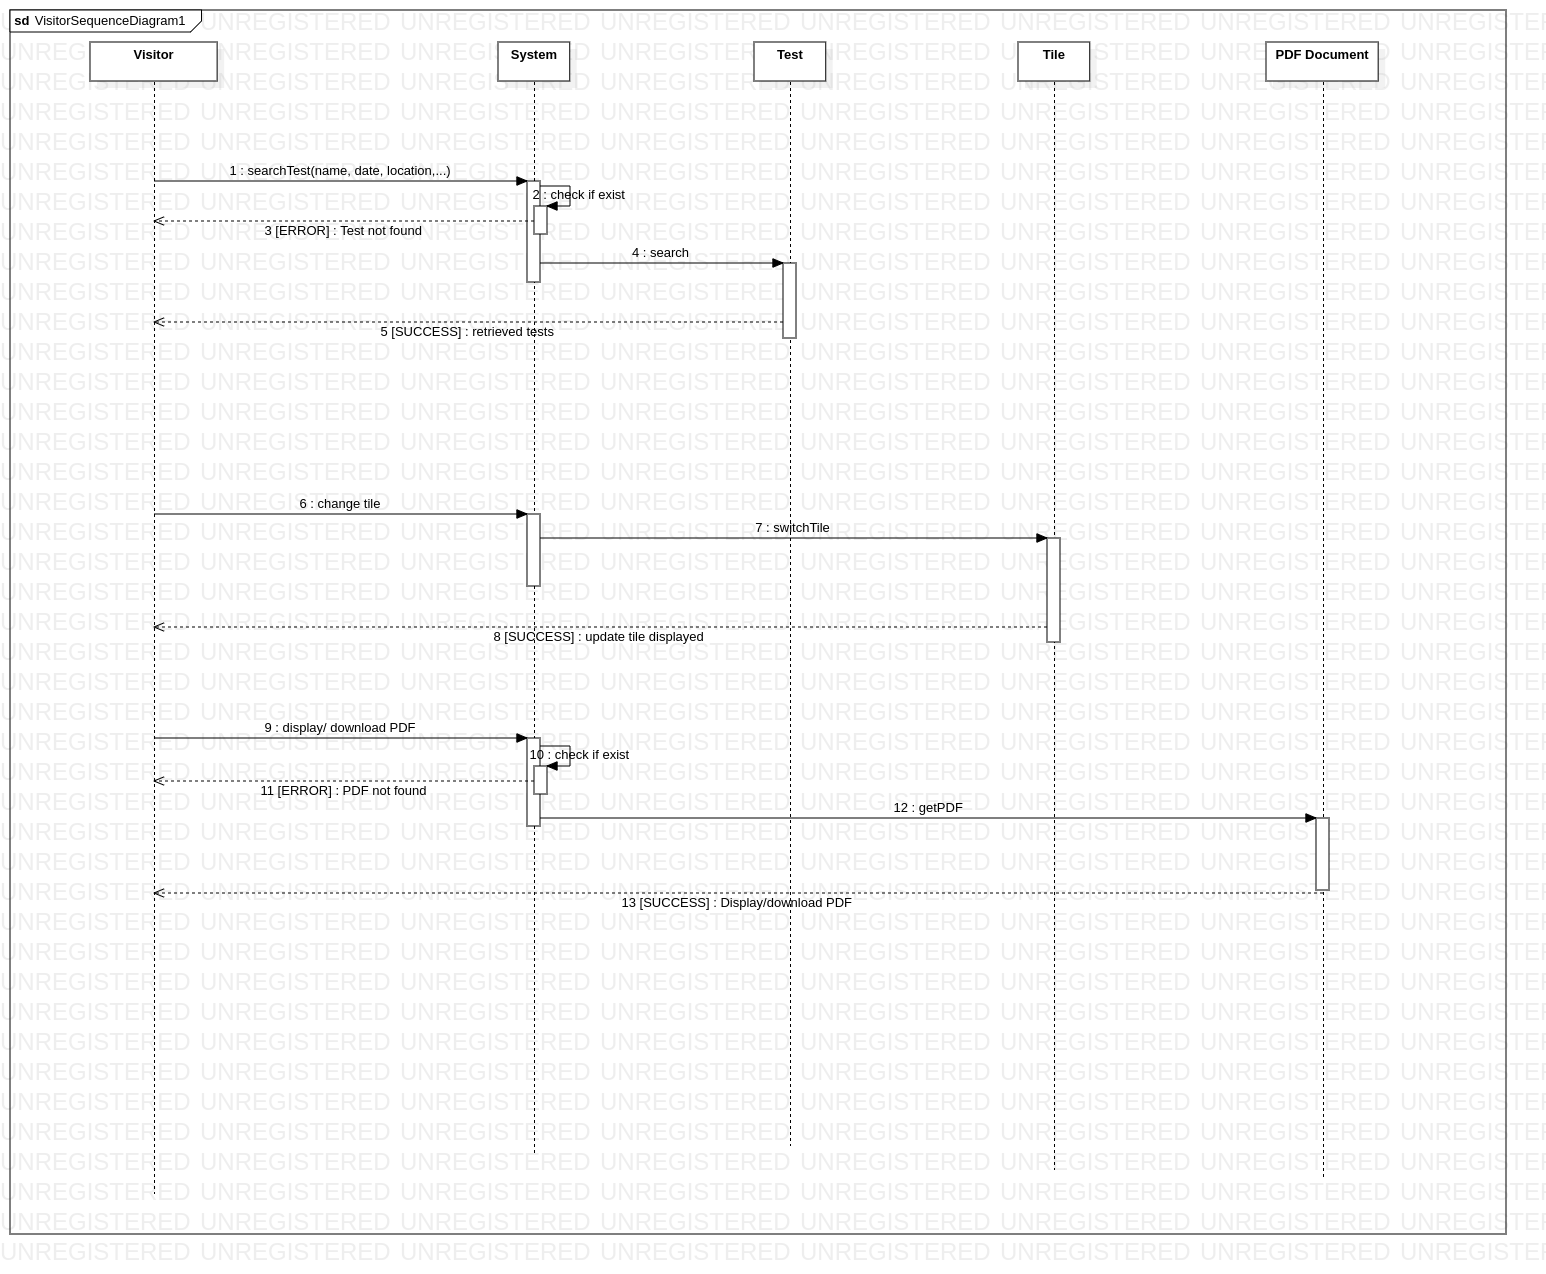
\includegraphics[width=1\textwidth]{images/Analyse_des_besoins/VisitorSequenceDiagram1.png}
        \caption{Diagramme des séquences : visiteur}
        \label{fig:VisitorSequenceDiagram1}
    \end{figure}
        
 